\subsubsection{Sit}

Se tiene cualitativamente las m\'ismas caracter\'isticas que en el caso anterior, con la diferencia que en este caso $ h:= p_v + 2(D_i -1) p_d$, y por ende para $\phi \in ]2(D_i - 1) p_d , p_V + 2(D_i -1)p_d[$ tendr\'iamos un comportamiento mon\'ontono para $f_{sit}$ y la existencia de un m\'aximo para $f_{grazing}$.\\

La figura \ref{fig:f1Sit} muestra las semejanzas con el caso anterior, salvo la diferencia que en este caso $k^*>1$ para el caso $3D$ y adem\'as alcanza un valor m\'as alto que el caso $2D$.\\
En general tenemos que $ k^*_{Sit} > k^*_{grazing}$ .

\begin{figure}
\begin{center}
 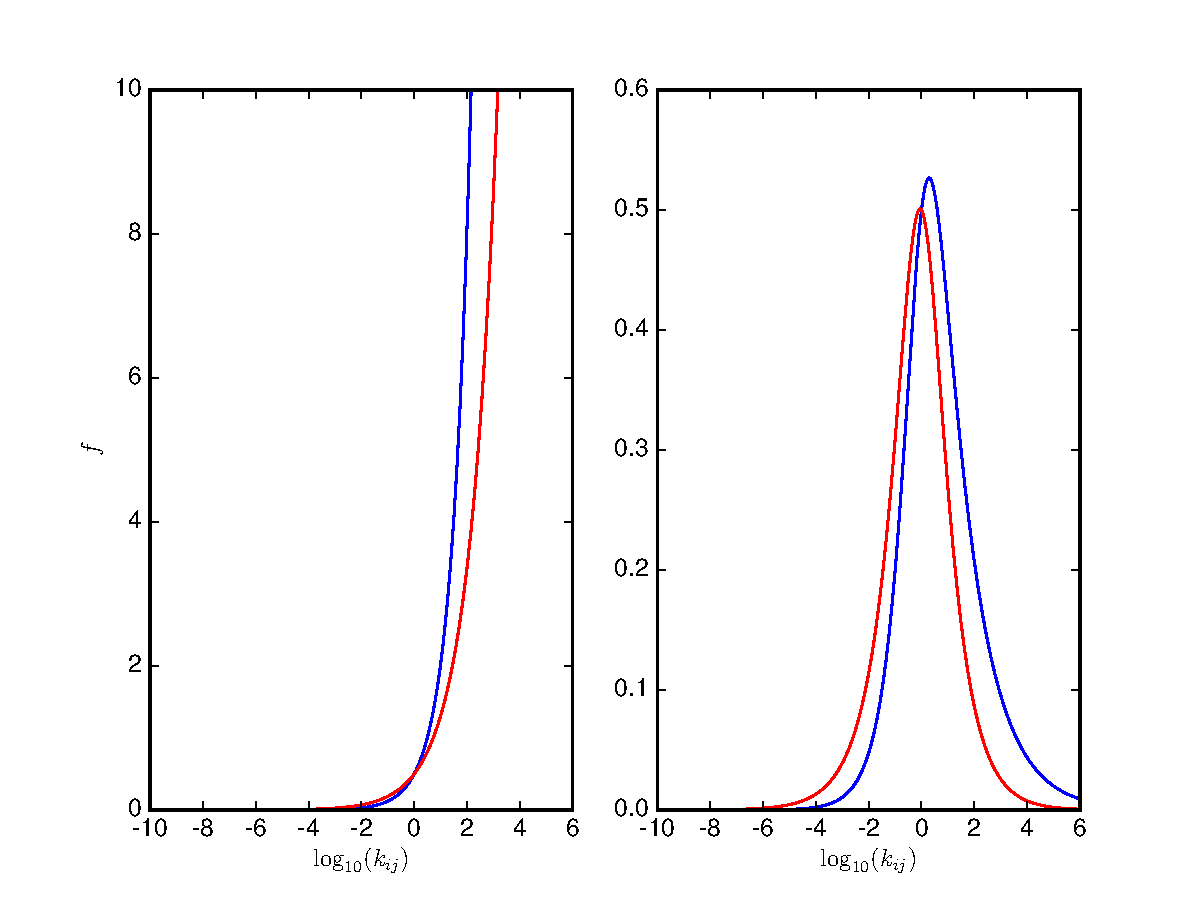
\includegraphics[width=0.9\textwidth]{./Plots/f1Sit.pdf}
 \caption[$f_1, Sit$]{$f$ en funci\'on a $k_{ij}$, con $a =1$, para el caso de una estrategia de forrajeo \emph{Sit-and-Wait}, las dem\'as especificaciones se comparten con la figura \ref{fig:f1Grazing}}
 \label{fig:f1Sit} 
\end{center}
\end{figure}

